%Template_made_by_SGjTeX

\documentclass[a4paper,13pt]{book}
\usepackage[utf8]{inputenc}     
\usepackage[T1]{fontenc}
\usepackage{amsmath,amsthm, amssymb,xcolor,amsfonts,mathrsfs} 
\usepackage[left=2.5cm,right=2.5cm,top=2.5cm,bottom=2.5cm]{geometry}
\usepackage[french]{babel}
\everymath{\displaystyle} 
\usepackage{hyperref}
%\usepackage{"./tpack"}

\usepackage{mathptmx}

\usepackage{mathtools}
\DeclarePairedDelimiter\ceil{\lceil}{\rceil}
\DeclarePairedDelimiter\floor{\lfloor}{\rfloor}
\usepackage{enumitem}
\usepackage[explicit]{ titlesec}
\usepackage{fancybox}
%\usepackage{thmbox}   
%================================ 
\usepackage{fancyhdr}
\usepackage{fancybox}

\usepackage{xcolor}
\pagestyle{fancy}
\fancyhf{} 

%\fancyfoot[RO,LE]{\rightmark} 

\cfoot{\thepage}
\lfoot{}
\renewcommand{\chaptermark}[1]{\markboth{#1}{}}
%===============================
\newtheorem{definition}{Définition}[section]
\newtheorem{theo}{Théorème}[section]
\newtheorem{pro}{Proposition}[section] 
\newtheorem{cor}{Corollaire}[section]
\newtheorem{lem}{Lemme}[section]
\newtheorem{rem}{Remarque}[section]

\definecolor{gris}{gray}{0.9}
\definecolor{perfectorange}{RGB}{255,165,20}
\definecolor{darkblue}{RGB}{25,25,100}
\definecolor{darkkblue}{RGB}{0,0,50}
\definecolor{darkred}{RGB}{180,0,0}
\definecolor{green_identifiers}{RGB}{00,80,00}
\definecolor{blue_know}{RGB}{00,20,20}
\definecolor{orange_comments}{RGB}{214, 161, 126}
\definecolor{red_keywords}{RGB}{215, 103, 129}
\definecolor{black_strings}{RGB}{50, 50, 50}
%utilis� dans la partie analyse
\definecolor{fond}{rgb}{.55,.55,.92}
%fin creation couleurs
% Définir le théorème avec couleur rouge
\newtheorem{danger1}{Attention}[section]
\newenvironment{danger}{\begin{danger1}\color{darkred}}{\end{danger1}}

% Définir le théorème avec couleur verte
\newtheorem{know1}{A Savoir}[section]
\newenvironment{know}{\begin{know1}\color{blue_know}}{\end{know1}}

\renewcommand{\footrulewidth}{1pt} 
\renewcommand{\thesection}{\arabic{section}}
\renewcommand{\thesubsection}{\thesection.\arabic{subsection}}
\renewcommand{\thesubsubsection}{\thesubsection.\arabic{subsubsection}}

\newcommand{\Hrule}{
	\rule{\linewidth}{0.5mm}
}
\newcommand\justify{%
  \let\\\@centercr
  \rightskip\z@skip
  \leftskip\z@skip}
%%===exercices 
%\newcounter{ex}
\newenvironment{exe}% exple \begin{exe}...\end{exe}
{\refstepcounter{ex}%
	\par\noindent
	{\underline{\bfseries{Exercice \theex \hspace*{0.009 cm} :}} }
	\mdseries
	\slshape}
{\par
	\medskip}
%====exemples
\newcounter{exple}
\newenvironment{exple}
{\refstepcounter{exple}%
	\par\noindent
	{\underline{\bfseries{Exemple  :}} }
	\mdseries
	\slshape}
{\par
	\medskip}
%====preuve
%\newenvironment{proof}
%{\rmfamily\mdseries{\bfseries Preuve : }}
%{\hfill$\blacksquare$}
%======
\renewcommand{\baselinestretch}{1.3}  

%%%%%%%%%%%%%%%%%%%%%%%%%%%%%%%%%

\newcommand{\ps}[2]{\left\langle #1 ,#2 \right\rangle  }
%%%%%%%%%%%%%%%%%%%%%% 
\let\cleardoublepage\clearpage 

\usepackage[explicit]{titlesec}
\usepackage{minitoc}
\renewcommand{\mtctitle}{Plan}
\usepackage[most]{tcolorbox}
\newcommand\mychapter{\titleformat{\chapter}[block]{}{}{0pt}{\centering\hrule height 5pt
		\vglue-1.1 \baselineskip
		\tcbox[enhanced,colback=white,frame code={}]{\bfseries\chaptername\hskip2mm \thechapter}
		\bigskip
		\vglue-3mm\hrule \vglue3mm
		{\huge \bfseries ##1}\vglue3mm\hrule
	}[]\chapter}
\dominitoc
\usepackage{caption}
\usepackage{listings}

%%configuration de listings
\definecolor{codegreen}{rgb}{0,0.6,0}
\definecolor{codegray}{rgb}{0.5,0.5,0.5}
\definecolor{codepurple}{rgb}{0.58,0,0.82}
\definecolor{backcolour}{rgb}{0.99,0.99,0.97}

\lstdefinestyle{mystyle}{
    backgroundcolor=\color{backcolour},
    commentstyle=\color{codegreen},
    keywordstyle=\color{magenta},
    numberstyle=\tiny\color{codegray},
    stringstyle=\color{codepurple},
    basicstyle=\ttfamily\footnotesize,
    breakatwhitespace=false,
    breaklines=true,
    captionpos=b,
    keepspaces=true,
    numbers=left,
    numbersep=5pt,
    showspaces=false,
    showstringspaces=false,
    showtabs=false,
    tabsize=4
}

\lstset{style=mystyle}

\definecolor{Zgris}{rgb}{238, 238, 238}

\newsavebox{\BBbox}
\newenvironment{DDbox}[1]{
\begin{lrbox}{\BBbox}\begin{minipage}{\linewidth}}
{\end{minipage}\end{lrbox}\noindent\colorbox{Zgris}{\usebox{\BBbox}} \\
[.5cm]}
\author{\bsc{DADA SIMEU Cédric Darel}}
\begin{document}
	\graphicspath{ {../Parallel_architecture/template_page_garde} }

\begin{center}
  
\includegraphics[scale=0.15]{logo.jpg}
\end{center}

{\vspace{7em}}

\begin{center}
  \begin{tabular}{|lp{5.0cm}lll|}
    \hline
    &  &  &  & {\small{2024/25}}\\
    &  &  &  & \\
    &  &  &  & \\
    \textbf{Nom:} & \bsc{DADA SIMEU Cédric Darel}
    
    \  &  &  & \\
    \textbf{Email:} & cedric-darel.dada@ensta-paris.fr
    
    \  &  &  & \\
    \textbf{Titre:} & Compte rendu TP 1
    
    
    \
    
    \  &  &  & \\
    \hline
  \end{tabular}
\end{center}

\

{\vspace{7em}}

\begin{center}
  \Large{{\textbf{STIC}}}
\end{center}

{\medskip}

\begin{center}
  ENSTA Paris, Institut Polytechnique de Paris
\end{center}

{\newpage}

\tableofcontents
\listoffigures
\newpage
\section{Produit matrice-matrice}
\subsection{Explication des résultats} 
\begin{table}[h!]
    \begin{center}
    \begin{tabular}{|c|c|c|}
        \hline
        Dimension & Temps CPU (s) & MFlops \\ \hline
        1023      & 12.5931       & 170.03 \\ \hline
        1024      & 17.6935       & 121.371 \\ \hline
        1025      & 12.8699       & 167.35 \\ \hline
    \end{tabular}
    \caption{Temps de calcul et performances en MFlops pour différentes dimensions de matrices.}
    \label{tab:perf_matrix}
\end{center}
\end{table}

Lorsque l'on exécute le programme avec différentes dimensions (1023, 1024, et 1025), on constate que : La dimension 1024  prend plus de temps que les autres.
    Cela est dû à l'alignement des données dans la mémoire cache. Lorsque la taille de la matrice correspond exactement à une puissance de deux (comme 1024), les lignes successives de la matrice peuvent se retrouver sur les mêmes lignes de cache, provoquant des conflits de cache (cache thrashing). Cela force le système à recharger fréquemment les lignes de cache, augmentant ainsi le temps d'exécution.
     

Solution proposée : 
Pour résoudre ce problème, on peut ajouter un padding (remplissage) aux matrices afin de décaler leur alignement en mémoire. Par exemple, ajoutez une ligne ou une colonne supplémentaire pour éviter ces conflits. 

\subsection{Première optimisation : Permutez les boucles jusqu’à obtenir un temps optimum }
  
Dans prodSubBlocks, les boucles sont organisées comme suit : 

\begin{table}[h!]
    \begin{center}
    \begin{tabular}{|c|c|c|}
        \hline
        Dimension & Temps CPU (s) & MFlops \\ \hline
        1023      & 12.5931       & 170.03 \\ \hline
        1024      & 17.6935       & 121.371 \\ \hline
        1025      & 12.8699       & 167.35 \\ \hline
    \end{tabular}
    \caption{Temps de calcul et performances en MFlops pour différentes dimensions de matrices (i,k,j).}
    \label{tab:perf_matrix_i,k_j}
\end{center}
\end{table}

\begin{table}[h!]
    \begin{center}
    \begin{tabular}{|c|c|c|}
        \hline
        Dimension & Temps CPU (s) & MFlops \\ \hline
        1023      & 1.46737       & 1459.21 \\ \hline
        1024      & 7.05546       & 304.372 \\ \hline
        1025      & 1.52632       & 1411.1  \\ \hline
    \end{tabular}
    \caption{Temps de calcul et performances en MFlops pour différentes dimensions de matrices (permutation i,j,k).}
    \label{tab:perf_matrix_i,j,k}
\end{center}
\end{table}

\begin{table}[h!]
    \begin{center}
    \begin{tabular}{|c|c|c|}
        \hline
        Dimension & Temps CPU (s) & MFlops \\ \hline
        1023      & 1.12464       & 1915.09 \\ \hline
        1024      & 1.1314       & 1892.53 \\ \hline
        1025      & 1.1196       & 1918.09 \\ \hline
    \end{tabular}
    \caption{Temps de calcul et performances en MFlops pour différentes dimensions de matrices (permutation j,k,i).}
    \label{tab:perf_matrix_first_j,k,i}
\end{center}
\end{table}

\begin{table}[h!]
    \begin{center}
    \begin{tabular}{|c|c|c|}
        \hline
        Dimension & Temps CPU (s) & MFlops \\ \hline
        1023      & 3.52183       & 584.697 \\ \hline
        1024      & 7.20673       & 297.983 \\ \hline
        1025      & 3.68359       & 1918.09 \\ \hline
    \end{tabular}
    \caption{Temps de calcul et performances en MFlops pour différentes dimensions de matrices (permutation j,i,k).}
    \label{tab:perf_matrix_first_j,i,k}
\end{center}
\end{table}

\begin{table}[h!]
    \begin{center}
    \begin{tabular}{|c|c|c|}
        \hline
        Dimension & Temps CPU (s) & MFlops \\ \hline
        1023      & 10.2218       & 209.474 \\ \hline
        1024      & 17.5939       & 122.059 \\ \hline
        1025      & 10.2415       & 1918.09 \\ \hline
    \end{tabular}
    \caption{Temps de calcul et performances en MFlops pour différentes dimensions de matrices (permutation k,i,j).}
    \label{tab:perf_matrix_first_k,i,j}
\end{center}
\end{table}

\begin{table}[h!]
    \begin{center}
    \begin{tabular}{|c|c|c|}
        \hline
        Dimension & Temps CPU (s) & MFlops \\ \hline
        1023      &  1.19066       & 1798.32 \\ \hline
        1024      & 1.03645       & 2071.97 \\ \hline
        1025      & 1.66156       & 1296.24 \\ \hline
    \end{tabular}
    \caption{Temps de calcul et performances en MFlops pour différentes dimensions de matrices (permutation k,j,i).}
    \label{tab:perf_matrix_first_k,j,i}
\end{center}
\end{table}
\clearpage
\paragraph{Optimisation} : 
Le stockage des matrices dans Matrix est basé sur un format colonne-major  (car m\_arr\_coefs[i+j*nbRows] accède d'abord aux colonnes). Pour maximiser l'utilisation du cache, il est préférable de permuter les boucles afin de parcourir les colonnes avant les lignes. La permutation optimale serait :\\

	\begin{lstlisting}[language=C]
        for (int j = iColBlkB; j < std::min(B.nbCols, iColBlkB + szBlock); j++) 
            for (int k = iColBlkA; k < std::min(A.nbCols, iColBlkA + szBlock); k++) 
                for (int i = iRowBlkA; i < std::min(A.nbRows, iRowBlkA + szBlock); ++i) 
                         C(i, j) += A(i, k) * B(k, j);
                    
    \end{lstlisting}

\paragraph{Explication} :  

    En parcourant les colonnes avant les lignes, nous minimisons les sauts en mémoire et exploitons pleinement les données chargées dans le cache. En effet, lorsqu'une donnée est chargée dans le cache, quelques unes de ses valeurs voisines y sont également chargées, et ainsi, en permutant la boucle de cette façon, nous récupérons ces données directement dans le cache.
    Cette permutation réduit significativement le temps d'exécution. Ainsi nous commençons par itérer sur j car j désigne toujours une colonne dans le calcul C(i, j) += A(i, k) * B(k, j). Ensuite nous continuons par k qui désigne en meme temps une ligne dans B et une colonne dans A. Nous terminons ensuite par i qui désigne une ligne dans A.

\subsection{Première parallélisation}
À l’aide d’OpenMP, parallélisons le produit matrice–matrice  


	\begin{lstlisting}[language=C]
        void prodSubBlocks(int iRowBlkA, int iColBlkB, int iColBlkA, int szBlock,
        const Matrix& A, const Matrix& B, Matrix& C) {
          #pragma omp parallel for
          for (int j = iColBlkB; j < std::min(B.nbCols, iColBlkB + szBlock); j++) {
              for (int k = iColBlkA; k < std::min(A.nbCols, iColBlkA + szBlock); k++) {
                  for (int i = iRowBlkA; i < std::min(A.nbRows, iRowBlkA + szBlock); ++i) {
                      C(i, j) += A(i, k) * B(k, j);
                  }
              }
          }
      }
    \end{lstlisting}

\paragraph{Explication}
\begin{itemize}
    \item La directive \#pragma omp parallel for nous permet de paralléliser la boucle externe sur j, distribuant les colonnes de C entre les threads.
    \item Ainsi, chaque thread calcule indépendamment les contributions pour ses colonnes attribuées, garantissant l'absence de conflits d'accès mémoire
\end{itemize}
\paragraph{Mesure de l'acclération}

\begin{table}[h!]
    \begin{center}
    \begin{tabular}{|c|c|c|}
        \hline
        Dimension & Temps CPU (s) & MFlops \\ \hline
        1023      & 1.30567       & 1639.92 \\ \hline
        1024      & 1.87234       & 1146.95 \\ \hline
        1025      & 1.43565        & 1500.21 \\ \hline
        Moyenne      & 1,537        & 1429,03 \\ \hline

    \end{tabular}
    \caption{Performances pour OMP\_NUM\_THREADS=1.}
\end{center}
\end{table}

\begin{table}[h!]
    \begin{center}
    \begin{tabular}{|c|c|c|}
        \hline
        Dimension & Temps CPU (s) & MFlops \\ \hline
        1023      & 0.384401       & 5570.22 \\ \hline
        1024      & 0.68271       & 3145.53 \\ \hline
        1025      & 0.46899        & 4592.38 \\ \hline
        Moyenne      & 0,512        & 4436,04 \\ \hline
    \end{tabular}
    \caption{Performances pour OMP\_NUM\_THREADS=4.}
\end{center}
\end{table}

\begin{table}[h!]
    \begin{center}
    \begin{tabular}{|c|c|c|}
        \hline
        Dimension & Temps CPU (s) & MFlops \\ \hline
        1023      & 0.358636       & 5970.4 \\ \hline
        1024      & 0.431726       & 4974.18 \\ \hline
        1025      & 0.423238        & 5088.82 \\ \hline
        Moyenne      & 0,4045        & 5344,47 \\ \hline
    \end{tabular}
    \caption{Performances pour OMP\_NUM\_THREADS=16.}
\end{center}
\end{table}.\\
Pour OMP\_NUM\_THREADS=4, on a une accélaration de $\frac{1,537}{0.512}=3.00$\\
Pour OMP\_NUM\_THREADS=16, on a une accélaration de $\frac{1,537}{0.4045}=3.80$

\subsection{Pourquoi il est possible d'améliorer encore les résultats?}

    Les performances peuvent être améliorées grâce au blocking  (ou blocage de cache).
    Diviser les matrices en sous-blocs permet de mieux exploiter les caches L1/L2.

\subsection{Deuxième optimisation : Optimisez le produit matrice–matrice par bloc}

Code : \\

	\begin{lstlisting}[language=C]
        namespace {
            void prodSubBlocks(int iRowBlkA, int iColBlkB, int iColBlkA, int szBlock,
                               const Matrix& A, const Matrix& B, Matrix& C) {
                for (int j = iColBlkB; j < std::min(B.nbCols, iColBlkB + szBlock); ++j) {
                    for (int k = iColBlkA; k < std::min(A.nbCols, iColBlkA + szBlock); ++k) {
                        const double b_kj = B(k, j); 
                        for (int i = iRowBlkA; i < std::min(A.nbRows, iRowBlkA + szBlock); ++i) {
                            C(i, j) += A(i, k) * b_kj;
                        }
                    }
                }
            }
            
            int findOptimalBlockSize(const Matrix& A, const Matrix& B) {
                std::vector<int> sizes = {16, 32, 64, 128, 256};
                double best_time = 1e9;
                int best_size = 64; 
            
                for (int sz : sizes) {
                    Matrix C(A.nbRows, B.nbCols, 0.0);
                    double start = omp_get_wtime();
                    
                    for (int I = 0; I < A.nbRows; I += sz) {
                        for (int J = 0; J < B.nbCols; J += sz) {
                            for (int K = 0; K < A.nbCols; K += sz) {
                                prodSubBlocks(I, J, K, sz, A, B, C);
                            }
                        }
                    }
                    
                    double duration = omp_get_wtime() - start;
                    if (duration < best_time) {
                        best_time = duration;
                        best_size = sz;
                    }
                }
                
                std::cout << "[OPTIM] Taille de bloc optimale: " << best_size << std::endl;
                return best_size;
            }
            } // namespace

            Matrix operator*(const Matrix& A, const Matrix& B) {
                Matrix C(A.nbRows, B.nbCols, 0.0);
                const int szBlock = 256;
            
                for (int I = 0; I < A.nbRows; I += szBlock) {       // Parcours lignes A
                    for (int J = 0; J < B.nbCols; J += szBlock) {   // Parcours colonnes B
                        for (int K = 0; K < A.nbCols; K += szBlock) { // Parcours commun
                            prodSubBlocks(I, J, K, szBlock, A, B, C);
                        }
                    }
                }
                return C;
            }
\end{lstlisting}

\paragraph{Conclusion : }Nous voyons que globalement, la taille optimale est \textbf{256}.
\paragraph{Commentaire : }
Notre machine (avec un Intel(R) Core(TM) i5-10210U) possède 6MiB de cache L3 et 1MiB répartis sur 4 cœurs en cache L2, soit environ 256KiB par cœur (voir fig \ref{tab:ls_topo} et \ref{tab:lscpu} ), et il se trouve que la taille 256 offre le meilleur compromis en termes de :
\begin{itemize}
    \item Réutilisation des données : Un bloc de taille 256$\times$256 en double précision (où chaque double occupe 8 octets) représente environ 256$\times$256$\times$8 = 524 288 octets (soit 512 KiB). Ce bloc (ou la combinaison de blocs issus de A, B et C) est dimensionné de façon à exploiter au mieux la capacité des caches de niveau L2 et L3.
    \item Amortissement du coût de chargement : Avec une taille de bloc bien choisie, une fois les sous-matrices chargées dans le cache, de nombreux calculs peuvent être effectués sans accéder à la mémoire principale.
    \item Optimisation pour la hiérarchie mémoire de votre machine : Les tailles de caches (L1, L2, L3) et la structure de la mémoire influencent fortement le choix d’un bloc optimal. Le fait que 256 apparaisse comme la meilleure taille dans vos tests expérimentaux est lié aux capacités spécifiques de votre ordinateur.
\end{itemize}

\begin{figure}[!h]
    \begin{center}
    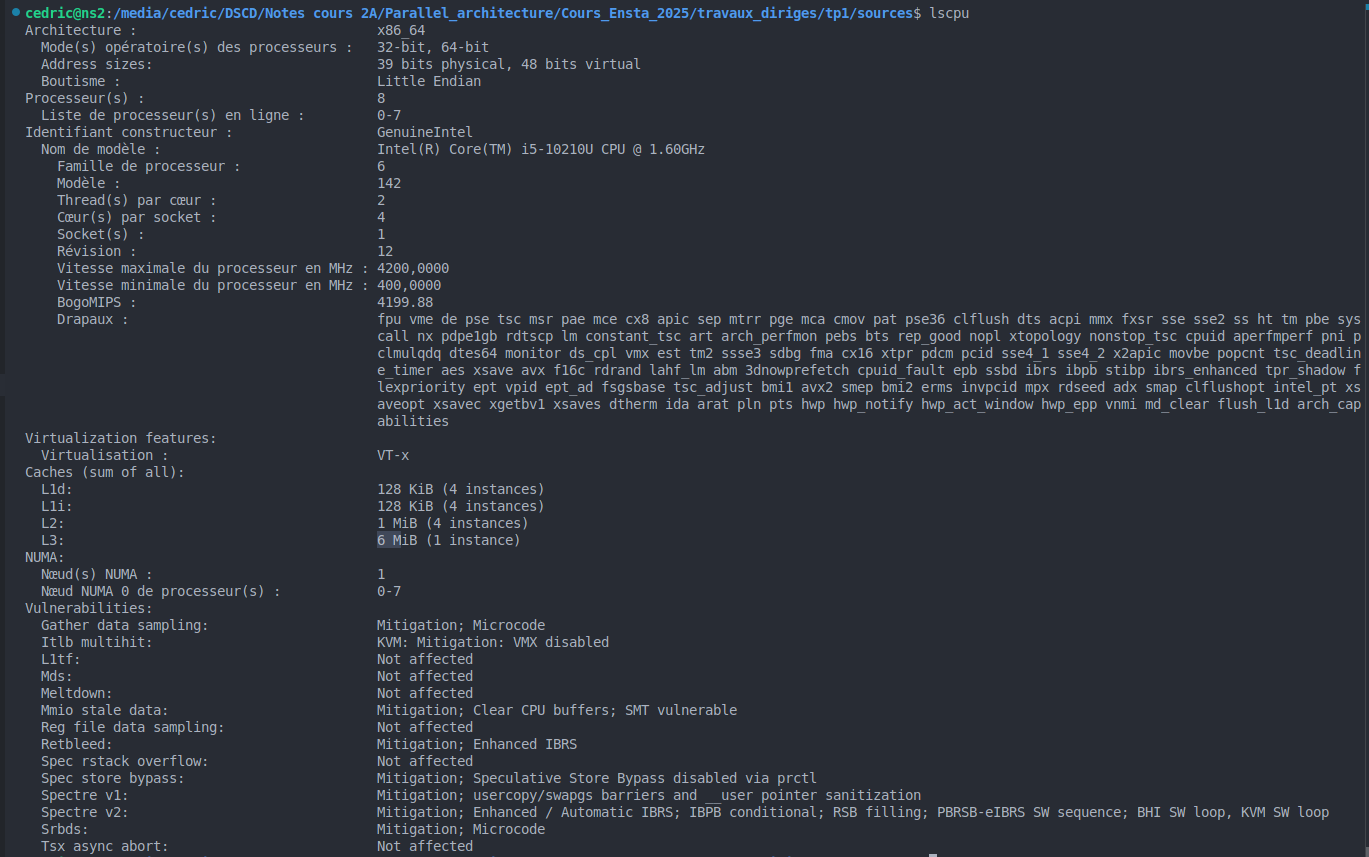
\includegraphics[scale=0.5]{images/lscpu.png}
    \caption{Résultat de la commande lscpu}
    \label{tab:lscpu}
\end{center}
\end{figure}


\begin{figure}[!h]
    \begin{center}
        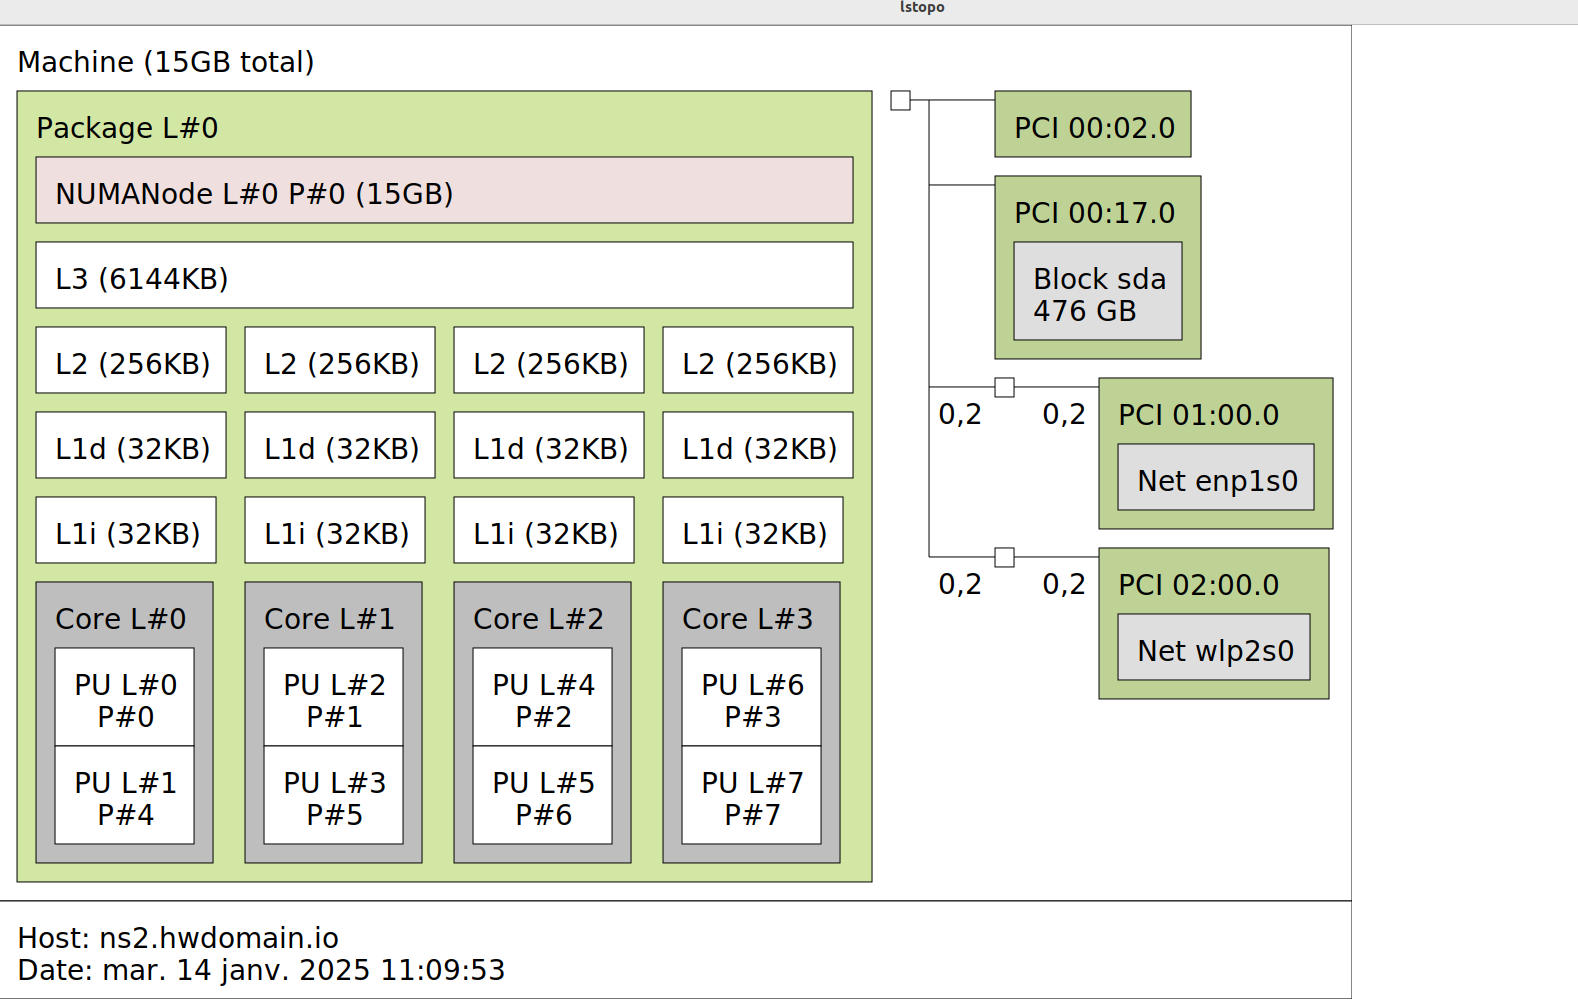
\includegraphics[scale=0.3]{images/lstopo.png}
        \caption{Résultat de la commande lstopo : Nous pouvons visualiser les tailles des caches}
        \label{tab:ls_topo}
    \end{center}
\end{figure}
\clearpage
\subsection{Comparer le temps pris par rapport au produit matrice–matrice "scalaire"}
    La version par bloc devrait être significativement plus rapide grâce à une meilleure utilisation des caches. Pour une taille de blocs de \textbf{256}, et un thread, nous avons une durée de moyenne (pour les dimensions 1023, 1024 et 1025) de \textbf{0,789 secondes}  contre \textbf{1,537 secondes} pour le produit matrice-matrice scalaire.

    \begin{table}
        \centering
        \caption{Temps d'exécution (secondes) pour N=1023-1025}
        \label{tab:small}
        \begin{tabular}{|c|c|c|c|c|c|}\hline
        Taille & 16 & 32 & 64 & 128 & 256 \\\hline
        1023 & 0.769 & 0.675 & 0.638 & 0.631 & \textbf{0.582} \\\hline
        1024 & 1.199 & \textbf{1.017} & 1.438 & 1.455 & 1.218 \\\hline
        1025 & 1.549 & 1.180 & 0.902 & 0.766 & \textbf{0.566} \\\hline
        2046  & 6.25 & 7.67 & 5.15 & 6.19 & \textbf{4.79} \\\hline
        2048 & 11.07 & 9.38 & 7.55 & 7.45 & \textbf{7.30} \\\hline
        2050 &  8.69 & 6.86 & 6.42 & 6.19 & \textbf{4.94} \\\hline
        \end{tabular}
        \caption{OMP\_NUM\_THREADS=1}
        \end{table}
\subsection{Parallélisation du produit matrice–matrice par bloc}


Code :  \\

	\begin{lstlisting}[language=C]
        Matrix operator*(const Matrix& A, const Matrix& B) {
            Matrix C(A.nbRows, B.nbCols, 0.0);
            const int szBlock = findOptimalBlockSize(A, B);
        
            #pragma omp parallel for
            for (int I = 0; I < A.nbRows; I += szBlock) {
                for (int J = 0; J < B.nbCols; J += szBlock) {
                    for (int K = 0; K < A.nbCols; K += szBlock) {
                        prodSubBlocks(I, J, K, szBlock, A, B, C);
                    }
                }
            }
            return C;
        }
\end{lstlisting}


\begin{table}[h!]
    \begin{center}
    \begin{tabular}{|c|c|c|}
        \hline
        Dimension & Temps CPU (s) & MFlops \\ \hline
        1023      & 0.625676       & 3422.21 \\ \hline
        1024      & 1.33775       & 1605.29 \\ \hline
        1025      & 1.24341        & 1732.16 \\ \hline
        Moyenne      & 1,06        & 2253,22 \\ \hline
    \end{tabular}
    \caption{Performances pour OMP\_NUM\_THREADS=1.}
\end{center}
\end{table}.

\begin{table}[h!]
    \begin{center}
    \begin{tabular}{|c|c|c|}
        \hline
        Dimension & Temps CPU (s) & MFlops \\ \hline
        1023      & 0.224386       & 9542.48 \\ \hline
        1024      & 0.23782       & 9029.87 \\ \hline
        1025      & 0.403212        & 5341.56 \\ \hline
        Moyenne      & 0,288        & 7971,30 \\ \hline
    \end{tabular}
    \caption{Performances pour OMP\_NUM\_THREADS=4.}
\end{center}
\end{table}.

\begin{table}[h!]
    \begin{center}
    \begin{tabular}{|c|c|c|}
        \hline
        Dimension & Temps CPU (s) & MFlops \\ \hline
        1023      & 0.255513       & 8380.01 \\ \hline
        1024      & 0.257188       &  8349.86 \\ \hline
        1025      & 0.228108        & 9441.95 \\ \hline
        Moyenne      & 0,247        & 8723,94 \\ \hline
    \end{tabular}
    \caption{Performances pour OMP\_NUM\_THREADS=16.}
\end{center}
\end{table}.

\paragraph{Mesure de l'accélération}
 Nous obtenons une accélération de \textbf{$\frac{1.06}{0.288}=3,68$} pour 4 threads et de \textbf{$\frac{1.06}{0.247}=4,29$} pour 16 threads.
\paragraph{Comparaison avec le produit matrice-matrice "scalaire"}
\begin{enumerate}
\item \textbf{ Observation} :
L'accélération parallèle est supérieure pour la version par blocs.
\item \textbf{Explications }:
    \begin{itemize}
    \item Réduction des conflits de cache : Les blocs isolent les zones mémoire travaillées par chaque thread → pas de false sharing.
    \item Localité mémoire préservée : Chaque thread travaille sur des sous-blocs contigus → meilleure utilisation du cache L1/L2.
    \item Granularité adaptée : La taille des blocs (ex: 256) équilibre charge de travail et utilisation du cache.
    \end{itemize}
\end{enumerate}
\textbf{Raison }:
Le surcoût de synchronisation est amorti par le volume de calcul dans chaque bloc.
 \subsection{Comparaison avec BLAS} 

 \begin{table}[h!]
    \begin{center}
    \begin{tabular}{|c|c|c|}
        \hline
        Dimension & Temps CPU (s) & MFlops \\ \hline
        1023      & 0.0473309       & 45238.9 \\ \hline
        1024      & 0.0609969       & 35206.4 \\ \hline
        1025      & 0.057084       & 37730 \\ \hline
        Moyenne & 0.055 & 39391,77 \\ \hline
    \end{tabular}
    \caption{Temps de calcul et performances en MFlops pour différentes dimensions de matrices obtenus avec Blas.}
    \label{tab:perf_matrix}
\end{center}
\end{table}
Les performances obtenues avec BLAS sont meilleures que celles obtenues avec notre produit matrice matrice par blocs parallélisé (16 threads). Le rapport moyen des performances $\approx \frac{0,247}{0.055} = 4.49$.

La meilleure version est celle de BLAS.
\section{Parallélisation MPI}
\subsection{Circulation d'un jeton dans un anneau.}


Code : \\

	\begin{lstlisting}[language=C]

        #include <stdio.h>
        #include <mpi.h>
        
        int main(int argc, char *argv[]) {
            int rank, nbp, token;
        
            /* Initialisation de l'environnement MPI */
            MPI_Init(&argc, &argv);
            MPI_Comm_rank(MPI_COMM_WORLD, &rank);
            MPI_Comm_size(MPI_COMM_WORLD, &nbp);
        
            /* On verifie qu'il y a au moins 2 processus */
            if(nbp < 2) {
                if(rank == 0)
                    fprintf(stderr, "Ce programme necessite au moins 2 processus.\n");
                MPI_Finalize();
                return 1;
            }
        
            /* Processus de rang 0 initialise le jeton et l'envoie au processus de rang 1 */
            if (rank == 0) {
                token = 1;  // initialisation du jeton
                printf("Processus %d envoie le jeton %d vers le processus 1\n", rank, token);
                MPI_Send(&token, 1, MPI_INT, 1, 0, MPI_COMM_WORLD);
                
                /* Processus 0 attend ensuite de recevoir le jeton venant du dernier processus */
                MPI_Recv(&token, 1, MPI_INT, nbp - 1, 0, MPI_COMM_WORLD, MPI_STATUS_IGNORE);
                printf("Processus %d a reçu le jeton %d depuis le processus %d\n", rank, token, nbp - 1);
            }
            else {
                /* Tous les autres processus reçoivent le jeton du processus precedent */
                MPI_Recv(&token, 1, MPI_INT, rank - 1, 0, MPI_COMM_WORLD, MPI_STATUS_IGNORE);
                token++;  // incrementation du jeton
                printf("Processus %d a reçu le jeton et l'incremente à %d\n", rank, token);
        
                /* Envoi du jeton au processus suivant.
                   Le processus nbp-1 envoie vers le processus 0 pour fermer l'anneau. */
                int dest = (rank + 1) % nbp;
                MPI_Send(&token, 1, MPI_INT, dest, 0, MPI_COMM_WORLD);
            }
        
            MPI_Finalize();
            return 0;
        }
        
\end{lstlisting}

\paragraph{Exécution}
\begin{enumerate}
    \item mpicc jeton.c -o jeton
    \item mpirun -np 4 ./jeton
\end{enumerate}
4 étant la valeur de nbp.\\
\textbf{Résultat}
\begin{itemize}
\item Processus 0 envoie le jeton 1 vers le processus 1
\item Processus 1 a reçu le jeton et l'incrémente à 2
\item Processus 2 a reçu le jeton et l'incrémente à 3
\item Processus 3 a reçu le jeton et l'incrémente à 4
\item Processus 0 a reçu le jeton 4 depuis le processus 3
\end{itemize}
\subsubsection{Calcul très approché de \pi}
\paragraph{Version séquentielle en c}.\\

	\begin{lstlisting}[language=C]
        /* pi_seq.c */
        #include <stdio.h>
        #include <stdlib.h>
        #include <time.h>
        #include <math.h>
        
        double approximate_pi(unsigned long nbSamples) {
            unsigned long nbDarts = 0;
            for (unsigned long i = 0; i < nbSamples; i++) {
                /* Generer un point dans [-1, 1] */
                double x = (double)rand() / RAND_MAX * 2.0 - 1.0;
                double y = (double)rand() / RAND_MAX * 2.0 - 1.0;
                if (x*x + y*y <= 1.0)
                    nbDarts++;
            }
            double ratio = (double)nbDarts / nbSamples;
            return 4.0 * ratio;
        }
        
        int main(void) {
            unsigned long nbSamples = 10000000UL; // par exemple 10 millions de points
            srand(time(NULL));
            clock_t tdeb = clock();
            double pi = approximate_pi(nbSamples);
            clock_t tfin = clock();
            double temps = (double)(tfin - tdeb) / CLOCKS_PER_SEC;
            printf("Approximation de pi (sequentiel) = %f\n", pi);
            printf("Temps d'execution = %f secondes\n", temps);
            return 0;
        }
        
        
\end{lstlisting}

\paragraph{Paralléliser en mémoire partagée le programme séquentiel en C à l'aide d’OpenMP}.\\


	\begin{lstlisting}[language=C]
        /* pi_openmp.c */
        #include <stdio.h>
        #include <stdlib.h>
        #include <time.h>
        #include <math.h>
        #include <omp.h>
        
        double approximate_pi(unsigned long nbSamples) {
            unsigned long nbDarts = 0;
        
            #pragma omp parallel
            {
                unsigned int seed = time(NULL) ^ omp_get_thread_num(); 
                unsigned long localCount = 0;
                #pragma omp for
                for (unsigned long i = 0; i < nbSamples; i++) {
                    double x = (double)rand_r(&seed) / RAND_MAX * 2.0 - 1.0;
                    double y = (double)rand_r(&seed) / RAND_MAX * 2.0 - 1.0;
                    if (x*x + y*y <= 1.0)
                        localCount++;
                }
                #pragma omp atomic
                nbDarts += localCount;
            }
            double ratio = (double)nbDarts / nbSamples;
            return 4.0 * ratio;
        }
        
        int main(void) {
            unsigned long nbSamples = 10000000UL;
            double tdeb = omp_get_wtime();
            double pi = approximate_pi(nbSamples);
            double tfin = omp_get_wtime();
            printf("Approximation de pi (OpenMP) = %f\n", pi);
            printf("Temps d'execution = %f secondes\n", tfin - tdeb);
            return 0;
        }
        
\end{lstlisting}

\paragraph{Mesure de l'accélération (fig \ref{tab:pi_approximation})}
\begin{table}[h!]
    \centering
    \begin{tabular}{|c|c|c|c|}
        \hline
    \toprule
    \textbf{Nombre de threads} & \textbf{Approximation de $\pi$ (OpenMP)} & \textbf{Temps d'exécution (secondes)} & \textbf{Accélération}\\
    \midrule
    1 thread                  & 3.141976                                  & 0.118586        & 1                       \\\hline
    4 threads                 & 3.142339                                  & 0.055988         &    2,118061013                  \\\hline
    8 threads                 & 3.140559                                  & 0.054829           & 2,162833537                   \\\hline
    16 threads                 & 3.141930                                  &  0.04843           & 2,448606236                   \\\hline
    \bottomrule
    \end{tabular}
    \caption{Résultats de l'approximation de $\pi$ avec OpenMP pour différents nombres de threads.}
    \label{tab:pi_approximation}
    \end{table}

    \paragraph{Version en mémoire distribuée avec MPI en C}.\\
    \begin{lstlisting}[language=C][language=C, caption=Code source de \texttt{pi\_mpi.c}]
        /* pi_mpi.c */
        #include <stdio.h>
        #include <stdlib.h>
        #include <time.h>
        #include <math.h>
        #include <mpi.h>
        
        int main(int argc, char *argv[]) {
            int rank, nbp;
            MPI_Init(&argc, &argv);
            MPI_Comm_rank(MPI_COMM_WORLD, &rank);
            MPI_Comm_size(MPI_COMM_WORLD, &nbp);
        
            unsigned long nbSamplesTotal = 10000000UL;
            /* Chaque processus traite une portion des echantillons */
            unsigned long nbSamples = nbSamplesTotal / nbp;
            unsigned long nbDarts_local = 0;
        
            /* Utiliser une graine differente pour chaque processus */
            unsigned int seed = time(NULL) ^ rank;
        
            double tdeb = MPI_Wtime();
            for (unsigned long i = 0; i < nbSamples; i++) {
                double x = (double)rand_r(&seed) / RAND_MAX * 2.0 - 1.0;
                double y = (double)rand_r(&seed) / RAND_MAX * 2.0 - 1.0;
                if (x*x + y*y <= 1.0)
                    nbDarts_local++;
            }
        
            unsigned long nbDarts_total = 0;
            MPI_Reduce(&nbDarts_local, &nbDarts_total, 1, MPI_UNSIGNED_LONG, MPI_SUM, 0, MPI_COMM_WORLD);
            double tfin = MPI_Wtime();
        
            if (rank == 0) {
                double ratio = (double)nbDarts_total / (nbSamples * nbp);
                double pi = 4.0 * ratio;
                printf("Approximation de pi (MPI) = %f\n", pi);
                printf("Temps d'execution (MPI) = %f secondes\n", tfin - tdeb);
            }
        
            MPI_Finalize();
            return 0;
        }        
        
\end{lstlisting}

\paragraph{Mesure de l'accélération (fig \ref{tab:pi_mpi})}


    \begin{table}[h!]
        \centering
        \begin{tabular}{|c|c|c|c|}
        \hline
        \textbf{Nombre de processus} & \textbf{Approximation de $\pi$ (MPI)} & \textbf{Temps d'exécution (secondes)} & \textbf{Accélération} \\
        \hline
        1                           & 3.141547                              & 0.168330                  & 1 \\\hline
        2                           & 3.141825                              & 0.084710                 &    1,98713257          \\\hline
        4                           & 3.142389                              & 0.072163                   &     2,332635838       \\\hline
        6                           & \textit{Erreur}                       & \textit{Non disponible}      & Non disponible         \\\hline
        8                           & \textit{Erreur}                       & \textit{Non disponible}      & Non disponible         \\\hline
        \end{tabular}
        \caption{Résultats de l'approximation de $\pi$ avec MPI pour différents nombres de processus.}
        \label{tab:pi_mpi}
        \end{table}
    
    \paragraph{Commentaire }
    Causes des erreurs : 
    \item Nombre de slots disponibles insuffisant
    \begin{itemize}
    \item Open MPI utilise le concept de slots pour allouer des processus. Un slot correspond à une unité d'allocation (généralement un cœur ou un thread).
    \item Notre processeur (Intel Core i5-10210U) a 4 cœurs physiques et 8 threads logiques (grâce à la technologie Hyper-Threading (fig \ref{tab:lscpu})).
    \item Par défaut, Open MPI limite le nombre de slots au nombre de cœurs physiques ou threads disponibles. Si on essaie de lancer plus de processus que de slots disponibles, l'erreur se produit.
    \end{itemize}
\paragraph{Version MPI en python avec mpi4py}.\\

	\begin{lstlisting}[language=C]
        #!/usr/bin/env python3
        # pi_mpi.py
        from mpi4py import MPI
        import time, numpy as np
        
        comm = MPI.COMM_WORLD
        rank = comm.Get_rank()
        size = comm.Get_size()
        
        nb_samples_total = 40_000_000
        nb_samples = nb_samples_total // size  # repartition uniforme des echantillons
        
        # Debut de la mesure de temps (commence avant le calcul)
        start = MPI.Wtime()
        
        # Chaque processus initialise sa graine pour générer des nombres aleatoires différents
        np.random.seed(int(time.time()) ^ rank)
        
        # Generation des points aleatoires dans [-1, 1] pour x et y
        x = np.random.uniform(-1, 1, nb_samples)
        y = np.random.uniform(-1, 1, nb_samples)
        
        # Compter le nombre de points tombant dans le cercle unite
        local_count = np.count_nonzero(x*x + y*y <= 1.0)
        
        # Réduire les resultats de tous les processus (somme)
        total_count = comm.reduce(local_count, op=MPI.SUM, root=0)
        
        # Fin de la mesure de temps
        end = MPI.Wtime()
        
        # Le processus maitre calcule l'approximation de pi et affiche le temps d'execution
        if rank == 0:
            approx_pi = 4.0 * total_count / nb_samples_total
            print(f"Approximation de pi (mpi4py) = {approx_pi}")
            print(f"Temps d'execution = {end - start} secondes")
        
        
\end{lstlisting}

\begin{table}[h!]
    \centering
    \begin{tabular}{|c|c|c|c|}
    \toprule
    \hline
    \textbf{Nombre de processus} & \textbf{Approximation de $\pi$ (MPI)} & \textbf{Temps d'exécution (secondes)} & \textbf{Accélération}\\
    \midrule    
    \hline
    1                           & 3.141979                              & 1.43688583   & 1                              \\\hline
    2                           & 3.1421147                              & 0.709724572     &    2,024568243                       \\\hline
    4                           & 3.1417664                              & 0.684759401      &     2,098380581                    \\\hline
    6                           & \textit{Erreur}                       & \textit{Non disponible}    & Non disponible            \\\hline
    8                           & \textit{Erreur}                       & \textit{Non disponible}    & Non disponible           \\\hline
    \bottomrule
    \end{tabular}
    \caption{Résultats de l'approximation de $\pi$ avec MPI pour différents nombres de processus.}
    \label{tab:pi_mpi_py}
    \end{table}

\subsection{Diffusion d'un entier dans un réseau hypercube.  }
Code :  \\


	\begin{lstlisting}[language=C]
        #include <stdio.h>
        #include <stdlib.h>
        #include <mpi.h>
        
        int main(int argc, char* argv[]) {
            int rank, nbp, d;
            MPI_Init(&argc, &argv);
            MPI_Comm_rank(MPI_COMM_WORLD, &rank);
            MPI_Comm_size(MPI_COMM_WORLD, &nbp);
        
            // Determination de la dimension d :
            // Si un argument est fourni, on l'utilise ; sinon, on deduit d a partir du nb de processus.
            if (argc > 1) {
                d = atoi(argv[1]);
            } else {
                // Deduire d si nbp est une puissance de 2.
                d = 0;
                int tmp = nbp;
                while (tmp > 1) {
                    if (tmp % 2 != 0) {
                        if (rank == 0)
                            fprintf(stderr, "Erreur : Le nombre de processus doit etre une puissance de 2.\n");
                        MPI_Finalize();
                        exit(EXIT_FAILURE);
                    }
                    tmp /= 2;
                    d++;
                }
            }
        
            // Verification : le nombre de processus doit etre 2^d.
            if (nbp != (1 << d)) {
                if (rank == 0)
                    fprintf(stderr, "Erreur : Pour un hypercube de dimension %d, il faut 2^d processus (ici %d processus).\n", d, nbp);
                MPI_Finalize();
                exit(EXIT_FAILURE);
            }
        
            int token;  // le jeton a diffuser
            double tdeb, tfin;
            
            // Mesurer le temps de diffusion
            tdeb = MPI_Wtime();
        
            // 1. Cas de l'hypercube de dimension 1 (2 processus) :
            //    - Si d vaut 1, alors seul 2 processus sont utilises.
            //    - Le processus 0 initialise et envoie au processus 1.
            // Ce meme algorithme fonctionne pour d = 2, d = 3 et d = d general.
            if (rank == 0) {
                token = 12345;  // valeur choisie par le programmeur
            }
            
            // Diffusion dans un hypercube en d etapes.
            // Pour chaque etape i, chaque processus echange avec son partenaire defini par rank xor (1 << i).
            for (int i = 0; i < d; i++) {
                int partner = rank ^ (1 << i);
                if (rank < partner) {
                    // Le processus avec un rang plus faible envoie d'abord
                    MPI_Send(&token, 1, MPI_INT, partner, 0, MPI_COMM_WORLD);
                } else {
                    // Celui avec le rang plus eleve recoit
                    MPI_Recv(&token, 1, MPI_INT, partner, 0, MPI_COMM_WORLD, MPI_STATUS_IGNORE);
                }
            }
            
            tfin = MPI_Wtime();
        
            // Affichage : chaque processus affiche la valeur recue et le temps de diffusion.
            printf("Processus %d : token = %d, temps de diffusion = %f secondes\n", rank, token, tfin - tdeb);
        
            MPI_Finalize();
            return 0;
        }
        
\end{lstlisting}
\textbf{mpirun -np 4 ./compute\_hypercube 2}
\begin{itemize}
\item Processus 0 : token = 12345, temps de diffusion = 0.000027 secondes
\item Processus 1 : token = 12345, temps de diffusion = 0.000085 secondes
\item Processus 2 : token = 12345, temps de diffusion = 0.000027 secondes
\item Processus 3 : token = 12345, temps de diffusion = 0.000116 secondes
\end{itemize}
\end{document}